\begin{blocksection}
\question Write a function, \lstinline$replace_x$ that takes in a tree, \lstinline$t$, and returns a new tree with all
labels \lstinline$x$ replaced with 0.

For example, if we called \lstinline$replace_x(t, 2)$ on the following tree:

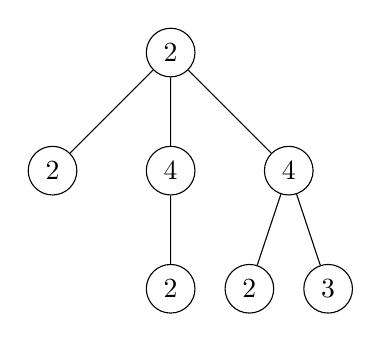
\begin{tikzpicture}[scale=1, transform shape]
\tikzstyle{level 2}=[sibling distance=10mm]
    \node [circle, draw] (z){$2$}
        child {node [circle, draw] (a) {$2$}}
        child {node [circle, draw] (d) {$4$}
            child {node [circle, draw] (g) {$2$}}
        }
        child {node [circle, draw] (b) {$4$}
            child {node [circle, draw] (e) {$2$}}
            child {node [circle, draw] (f) {$3$}}
        };
\end{tikzpicture}

We would expect it to return

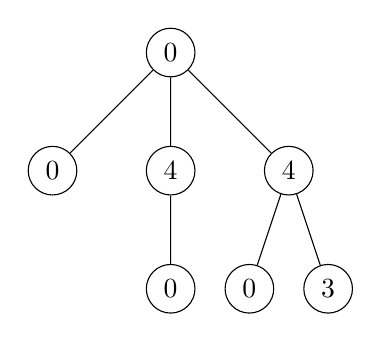
\begin{tikzpicture}[scale=1, transform shape]
\tikzstyle{level 2}=[sibling distance=10mm]
    \node [circle, draw] (z){$0$}
        child {node [circle, draw] (a) {$0$}}
        child {node [circle, draw] (d) {$4$}
            child {node [circle, draw] (g) {$0$}}
        }
        child {node [circle, draw] (b) {$4$}
            child {node [circle, draw] (e) {$0$}}
            child {node [circle, draw] (f) {$3$}}
        };
\end{tikzpicture}

\begin{lstlisting}
def replace_x(t, x):
    







\end{lstlisting}

\begin{solution}
\begin{lstlisting}
   new_branches = [replace_x(b, x) for b in branches(t)]
   if label(t) == x:
        return tree(0, new_branches)
   return tree(label(t), new_branches)
\end{lstlisting}

Here, we construct and return a new tree. First, we make 
a new list of branches where each branch is the same
as the previous branch but all occurrences of x have been
replaced with 0 (this is what the output of \lstinline$replace_x$
is defined to be.)
\newline
\newline
If the label of our tree is equal to x, we will additionally need 
to "replace" our current label with 0 in the tree we return. Otherwise,
we can keep our previous label.
\newline
\newline
These two steps guarantee that each occurrence of x is replaced.
\newline
\newline
We do not need a base case here, as if we are at a leaf, the list
comprehension we use to create the new branches will evaluate to an 
empty list. Then we will either return \lstinline$tree(0, [])$ or
\lstinline$tree(label(t), [])$ as appropriate. 
\end{solution}
\end{blocksection}
